\documentclass[activite]{thedocument}
\usepackage{tkz-euclide}
\startdatakeys
\source{}
\cycle{}
\competencesDuSocle{}
\connaissancesRequises{}
\competencesTravaillees{}
\enddatakeys
\begin{document}
    \noindent
    Dans chaque cas, écrire l'expression numérique donnant l'aire du rectangle $ABCD$.\par
    \begin{enumerate}
        \item\hskip30pt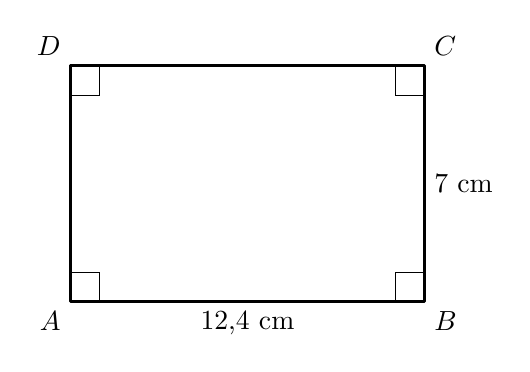
\begin{tikzpicture}[scale=1.5]
            \tkzDefPoint(0,0){A}
            \tkzDefPoint(3,0){B}
            \tkzDefPoint(3,2){C}
            \tkzDefPoint(0,2){D}
            \tkzLabelPoints[below left](A)
            \tkzLabelPoints[below right](B)
            \tkzLabelPoints[above right](C)
            \tkzLabelPoints[above left](D)
            \tkzDrawPolygon[line width=1pt](A,B,C,D)
            \tkzMarkRightAngles(A,B,C B,C,D C,D,A D,A,B)
            \tkzDefMidPoint(A,B)
            \tkzGetPoint{M}
            \tkzDefMidPoint(C,B)
            \tkzGetPoint{N}
            \draw node[below]at(M){12,4 cm};
            \draw node[right]at(N){7 cm};
        \end{tikzpicture}\vskip30pt
        \item\hskip30pt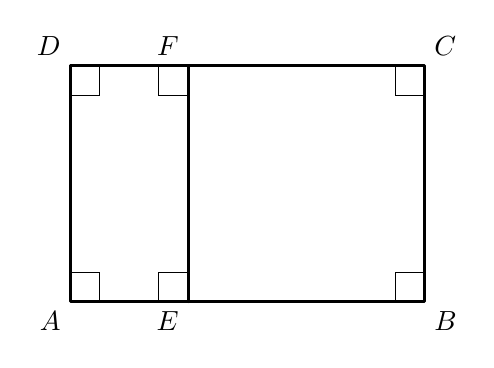
\begin{tikzpicture}[scale=1.5]
            \tkzDefPoint(0,0){A}
            \tkzDefPoint(3,0){B}
            \tkzDefPoint(3,2){C}
            \tkzDefPoint(0,2){D}
            \tkzDefPoint(1,0){E}
            \tkzDefPoint(1,2){F}
            \tkzLabelPoints[below left](A,E)
            \tkzLabelPoints[below right](B)
            \tkzLabelPoints[above right](C)
            \tkzLabelPoints[above left](D,F)
            \tkzDrawPolygon[line width=1pt](A,B,C,D)
            \tkzDrawSegment[line width=1pt](E,F)
            \tkzMarkRightAngles(A,B,C B,C,D C,D,A D,A,B A,E,F E,F,D)
        \end{tikzpicture}\vskip10pt
        \hskip30pt $AE=2,5$ m
        \hskip30pt $EB=5$ m
        \hskip30pt $DA=4,5$ m\vskip30pt
        \item\hskip30pt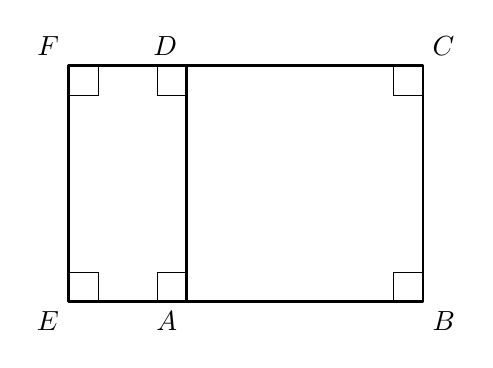
\begin{tikzpicture}[scale=1.5]
            \tkzDefPoint(0,0){E}
            \tkzDefPoint(3,0){B}
            \tkzDefPoint(3,2){C}
            \tkzDefPoint(0,2){F}
            \tkzDefPoint(1,0){A}
            \tkzDefPoint(1,2){D}
            \tkzLabelPoints[below left](E,A)
            \tkzLabelPoints[below right](B)
            \tkzLabelPoints[above right](C)
            \tkzLabelPoints[above left](D,F)
            \tkzDrawPolygon[line width=1pt](E,B,C,F)
            \tkzDrawSegment[line width=1pt](A,D)
            \tkzMarkRightAngles(E,B,C B,C,F C,F,E F,E,B E,A,D A,D,F)
        \end{tikzpicture}\vskip10pt
        \hskip30pt $AE=2,5$ m
        \hskip30pt $EB=12$ m
        \hskip30pt $CB=4,5$ m
    \end{enumerate}
    
\end{document}

